%% LyX 2.2.1 created this file.  For more info, see http://www.lyx.org/.
%% Do not edit unless you really know what you are doing.
\documentclass[12pt,english]{article}
\renewcommand{\familydefault}{\sfdefault}
\usepackage{geometry}
\geometry{verbose,tmargin=1in,bmargin=1in,lmargin=1cm,rmargin=1in}
\usepackage{float}
\usepackage{amsmath}
\usepackage{amsthm}
\usepackage{graphicx}

\makeatletter
%%%%%%%%%%%%%%%%%%%%%%%%%%%%%% Textclass specific LaTeX commands.
\numberwithin{equation}{section}
\numberwithin{figure}{section}

%%%%%%%%%%%%%%%%%%%%%%%%%%%%%% User specified LaTeX commands.
\date{ }
\newcommand*{\adt}{Linked List}
\setcounter{section}{1}

\makeatother

\usepackage{babel}
\usepackage{listings}
\renewcommand{\lstlistingname}{Listing}

\begin{document}

\title{Review: Function Pointers}
\maketitle

\section*{Overview}

This review will cover an introductory to function pointers. This
review covers the basic introductory material, that was provided in
other required courses. Pointers are a fundamental component that
must be integrated into the development of your labs and assignments
throughout the course. We will review the basic introduction to the
topic, including a ``Getting Started'' example, and some common
best practices.

\section*{Learning Outcomes}

Upon successful completion of this review, students should be able
to:
\begin{itemize}
\item describe the key benefits of pointers
\item explain the difference between referencing and dereferencing pointers
\item apply pointers to the development of an abstract data type
\item manage pointers to reduce memory leaks and errors
\end{itemize}

\section*{Introduction}

In this review, we will cover the basics of:
\begin{itemize}
\item function pointers
\end{itemize}

\section*{Getting Started}

Please ensure that you're comfortable with material on general C-Programming
and void pointers if required students should review notes from CIS{*}2500
or ask for additional materials from the instructor of 2520

\subsection*{Function Pointers}

A function pointer is similar to a regular pointer, except that it
holds the address of a function. Much like regular pointers function
pointers have a type, they must point to a function with a matching
declaration. Functions with matching declarations have identical return
types and the parameter lists matches, ie the data type of each parameter
the type and number of parameters. For instance:

\begin{lstlisting}[showstringspaces=false,tabsize=4,frame={T|B}]
	// Functions with matchings declarations
	int add( int a, int b );
	int sub( int c, int d );
	
	void sort( int* arr, int sizeOfArray);
	void reverse( int * arr, int sizeOfArray );
	
\end{lstlisting}

\medskip{}

If the functions have a different number of parameters, return types,
or the data type of each parameter is different the functions do not
match. To declare a function pointer use the following form:
\noindent \begin{center}
\begin{lstlisting}[showstringspaces=false,tabsize=4,frame={T|B}]
	ex) returnType (*functionName) ( parameters );
	
	void (*funcPtr)(int,char,int);
\end{lstlisting}
\par\end{center}

\medskip{}

Here we have a function pointer called funcPtr that has a return type
void, and a parameter list of size three with the order integer, char,
and integer. As this is just a declaration function does not point
to a function yet, it just describes what type of functions it can
point to. Let look at an example of pointing a function pointer at
a function.

\begin{lstlisting}[showstringspaces=false,tabsize=4,frame={T|B}]
	// a normal function to add two numbers
	int add( int a, int b )
	{
		return a+b;
	}
	
	int sub( int a, int b )
	{
		return a-b;
	}
	
	int main()
	{
		// Declare our function pointer
		int (*mathOperator)(int,int);
	
		// Just like with normal pointers,
		// points to the memory address of the add function
		mathOperator = &add;
	
		// Since we pointed to add, 
		// the add function is called, the result is 5
		int result = mathOperator(2,3);
	}
\end{lstlisting}

\medskip{}

A function pointer can be a pointer within your program but it can
also be a parameter in another function. In this next example, the
mathOperator is a parameter for another function and that gets called
on the other parameters. Two functions isGreater and isEqual are passed
into performOperation to demonstrate calling.

\begin{lstlisting}[showstringspaces=false,tabsize=4,frame={T|B}]
	// Create a function with three parameters 
	// two integeres and math operator
	int performOperation( int a, int b, int (*mathOperator) (int , int))
	{
		return mathOperator(a,b);
	}
	
	function isGreater( int a, int b)
	{
		return a>b;
	}
	
	function isEqual( int a, int b)
	{
		return a == b;
	}
	
	int main()
	{
		int a = 3, b= 6;
		int result = performOperator(a,b, isGreater);
		int result2 = performOperator(b,a, isEqual);
	}
\end{lstlisting}

For more on function pointers see the tutorial (http://www.cprogramming.com/tutorial/function-pointers.html)

\section*{Practical Example}

This section provides a brief introduction to the construction of
a Linked List Abstract Data Type (ADT). The example in Figure \ref{fig:LinkedListCode},
demonstrates the initial steps in creating a Single Linked List. In
the leftmost box, two structures are created for the ListNode and
the Improved List. The ListNode structure demonstrates a void pointer
for the data member and the ImprovedList structure demonstrates function
pointers for the destroyPtr. The code on the right-side demonstrate
two functions to create the List and destroy the list. The createList
function will receive a function pointer that indicates how stored
data will later be destroyed. The createList function simply stores
that pointer for later use when it is time to destroy the list. During
the creation of an ADT, such as the Linked List, we often pass function
pointers that describe how the ADT should handle the contained data
type. When the destroyList function is called it internally calls
the destroyPtr function pointer for each data member, this properly
free the heap memory for data stored in your node.

\begin{figure}[H]
\begin{centering}
\includegraphics[scale=0.5]{linkedListExample}\caption{\label{fig:LinkedListCode}Construction of a Linked List Node and
creating and destroying the list with a function pointer parameter.}
\par\end{centering}
\end{figure}


\section*{Best Practices}

Pointers, void pointers, and function pointers can take a bit of practice
to become confident using in your daily applications. A suggestion
when working with pointers is to remove some of the ugly and difficult
to read syntax that inheritance comes along with pointers. One suggestion
is to improve the readability of your code by using typedefs.

\begin{lstlisting}[showstringspaces=false,tabsize=4,frame={T|B}]
	/* 
	Pointers are more difficult to look at .... lets change that.
	Typedefs take the original name and making an alias for it.
	The form is: typedef oldName newName
	To improve the readability of void pointers, we can use
	*/
	typedef void* VoidPtr;
	
	/*
	Now this statement looks more like the variables
	we're used to....although you still have to manage the memory.
	*/
	VoidPtr myData;
	
	// Function pointers also have poor readability.
	// Create a function pointer called FunctionPtr
	typedef int (*FunctionPtr)(int,int);
	
	/*
	This creates a function pointer that returns 
	an int and has two integers as parameters, use it as follows:
	*/
	FunctionPtr myFunc = &add;
	myFunc(2,3); 
\end{lstlisting}

\end{document}
